\documentclass[conference]{IEEEtran}
\IEEEoverridecommandlockouts
% The preceding line is only needed to identify funding in the first footnote. If that is unneeded, please comment it out.
\usepackage{cite}
\usepackage{amsmath,amssymb,amsfonts}
\usepackage{algorithmic}
\usepackage{graphicx}
\usepackage{textcomp}
\usepackage{xcolor}
\usepackage{tabularx}
\usepackage{multirow}
\usepackage{graphics} % for pdf, bitmapped graphics files
\usepackage{subfig}
\usepackage{subcaption}
\usepackage{hyperref}
\usepackage{academicons}
\usepackage{xcolor}
\usepackage{listings}
\usepackage{tabularx} % Asegúrate de incluir este paquete

\usepackage{tikz}
\usetikzlibrary{shapes.geometric, arrows}

\usetikzlibrary{shapes.geometric, arrows}

\tikzstyle{startstop} = [rectangle, rounded corners, minimum width=3cm, minimum height=1cm,text centered, draw=black, fill=red!30]
\tikzstyle{process} = [rectangle, minimum width=3cm, minimum height=1cm, text centered, draw=black, fill=blue!30]
\tikzstyle{arrow} = [thick,->,>=stealth]


\def\BibTeX{{\rm B\kern-.05em{\sc i\kern-.025em b}\kern-.08em
		T\kern-.1667em\lower.7ex\hbox{E}\kern-.125emX}}

% Color Enlace
\definecolor{colorEnlace}{RGB}{0, 0, 0}
\hypersetup{
	colorlinks=true,
	linkcolor=colorEnlace,
	citecolor=colorEnlace,
	urlcolor=colorEnlace,
	pdfauthor={Davis Bremdow Salazar Roa},
	pdftitle={Sistemas Embebidos}
}
\definecolor{mybg}{rgb}{0.97,0.97,0.97}
\definecolor{mygray}{gray}{0.4}
\definecolor{mygreen}{rgb}{0,0.6,0}
\definecolor{myblue}{rgb}{0,0,0.8}
\definecolor{mypurple}{rgb}{0.58,0,0.82}
\definecolor{myred}{rgb}{0.7,0,0}

\lstdefinelanguage{MatlabEnhanced}{
	language=Matlab,
	morekeywords={[2]linspace,plot,title,xlabel,ylabel,legend,grid},
	morekeywords={[3]sin,cos,exp,log,sqrt},
	keywordstyle=\color{myblue}\bfseries,
	keywordstyle=[2]\color{mypurple},
	keywordstyle=[3]\color{myred},
	commentstyle=\color{mygreen}\itshape,
	stringstyle=\color{mygray},
	morecomment=[l]%
}

\lstset{
	language=MatlabEnhanced,
	backgroundcolor=\color{mybg},
	frame=single,
	basicstyle=\ttfamily\small,
	showstringspaces=false,
	numbers=none,              %
	xleftmargin=0pt,           %
	framexleftmargin=0pt,      
	framexrightmargin=0pt,
	framextopmargin=2pt,
	framexbottommargin=2pt,
	breaklines=true,
	tabsize=1,
}

% Control 
\usepackage{amsmath}
\begin{document}
	
	\title{Modulación Angular - PM, FM}
	\author{
		\makebox[\textwidth][c]{\large\textbf{Universidad Nacional de San Antonio Abad del Cusco}}\\
		\makebox[\textwidth][c]{\normalsize\textit{Escuela profesional de Ingeniería Electrónica}}\\
		\makebox[\textwidth][c]{\normalsize\textit{Laboratorio de Circuitos Electrónicos III}}\\
		\and
		\IEEEauthorblockN{Ing. Milton Velasquez Curo}
		\IEEEauthorblockA{Ingeniero Electrónico \\
			Cusco, Perú \\
			milton.velasquez@unsaac.edu.pe}
		\and
		\IEEEauthorblockN{Ruth Juana Espino Puma - 185746}
		\IEEEauthorblockA{Estudiante de Ingeniería Electrónica \\
			Cusco, Perú \\
			184657@unsaac.edu.pe}
		\and
		\IEEEauthorblockN{Davis Bremdow Salazar Roa - 200353}
		\IEEEauthorblockA{Estudiante de Ingeniería Electrónica \\
			Cusco, Perú \\
			200353@unsaac.edu.pe}
	}
	
	\maketitle
	\begin{abstract}
		La modulación es un proceso fundamental en las telecomunicaciones que consiste en variar una o más propiedades de una señal portadora (como amplitud, frecuencia o fase) en función de una señal de información o mensaje. Este proceso permite transmitir información a largas distancias de manera eficiente, minimizando interferencias y aprovechando mejor el espectro de frecuencias. Existen varios tipos de modulación, entre ellos la modulación en amplitud (AM), frecuencia (FM) y fase (PM), cada una con características y usos específicos según las necesidades del sistema de comunicación.
		
	\end{abstract}
	
	\begin{IEEEkeywords}
		Modulación, portadora, señal, índice de modulación, amplitud, frecuencia, fase, transmisión, espectro, distorsión.
	\end{IEEEkeywords}
	
	%% Contenido del documento
	\section{Modulación PM y FM}
	
	Una técnica adicional a la modulación de amplitud en la cual la señal de información modifica proporcionalmente este parámetro es la modulación angular la cual consiste en modificar el angulo en relación directa a la moduladora.
	
	A este tipo de procedimiento de forma matemática se puede describir de forma general en \ref{eq:mod-angular-general}
	
	\begin{equation}
		\Phi(t) = Acos\theta (t)
		\label{eq:mod-angular-general}
	\end{equation}
	
	Y en la cual el angulo $\theta(t)$ ahora es variable manteniendo constante la amplitud de la señal (reduciendo el ruido durante la transmisión de la señal).
	
	Finalmente en este tipo de modulación el angulo además se puede describir como en \ref{eq:mod-general-pm} y \ref{eq:mod-general-fm} para una señal PM y FM respectivamente.
	
	\begin{equation}
		\theta(t) = \omega_ct + k_pf(t) + \gamma_0
		\label{eq:mod-general-pm}
	\end{equation}
	
	\begin{equation}
		\theta(t) = \omega_ct + \int_0^t{k_pf(\tau) d\tau} + \gamma_0
		\label{eq:mod-general-fm}
	\end{equation}
	
	Para ejemplificar estos 2 conceptos, se hará uso de la señales de información mostradas en las figuras \ref{fig:moduladora-cuadrada} y \ref{fig:moduladora-triangularpng} para ambos tipos de modulación.
	
	\begin{figure}[h]
		\centering
		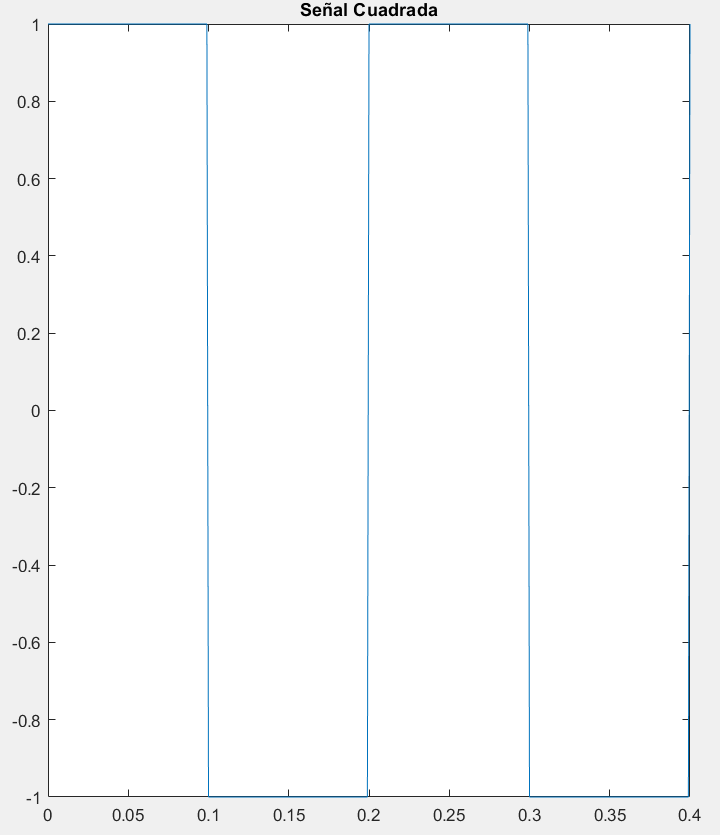
\includegraphics[width=0.35\textwidth]{media/moduladora-cuadrada}
		\caption{Señal cuadrada - Moduladora PM, FM}
		\label{fig:moduladora-cuadrada}
	\end{figure}
	
	\begin{figure}[h]
		\centering
		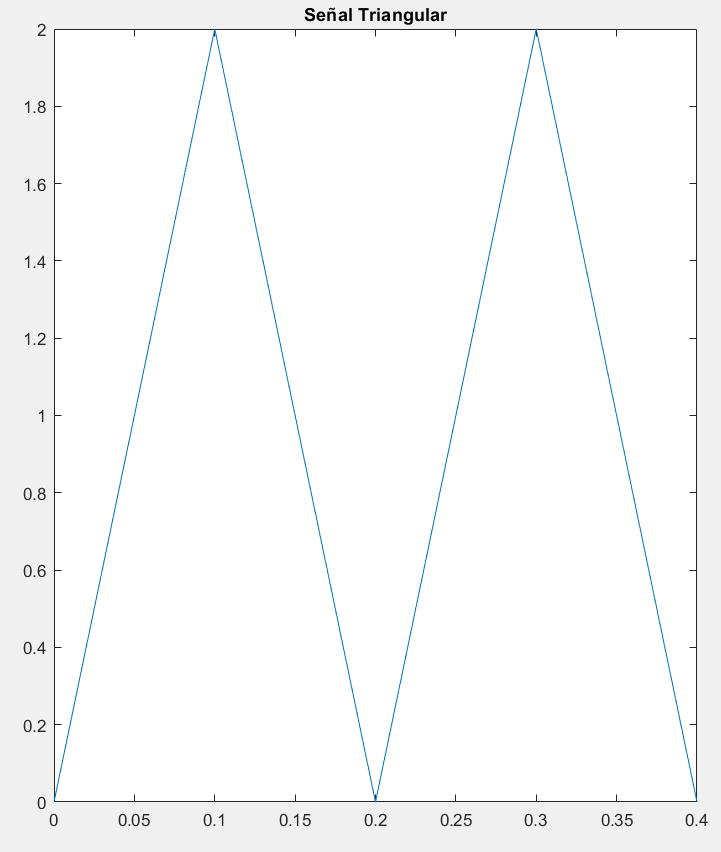
\includegraphics[width=0.35\textwidth]{media/moduladora-triangularpng}
		\caption{Señal triangular - Moduladora PM, FM}
		\label{fig:moduladora-triangularpng}
	\end{figure}
	
	Y en donde la señal triangular mostrada en la figura \ref{fig:moduladora-triangularpng} es la integral de la señal cuadrada mostrada en \ref{fig:moduladora-cuadrada}, definiendose ambas relaciones para medir posteriormente realizar una comparación entre ambos tipos de modulación.
	
	\section{ Modulación PM}
	
	Una característica fundamental de la modulación en fase (PM) consiste en relacionar la fase de la portadora de forma lineal con la señal de información, sin embargo este proceso aunque intuitivo, no difiere mucho de una modulación FM, debido a que como se muestra en \ref{eq:mod-fm} la única diferencia es la integral en la expresión para la moduladora.
	
	Obviando principalmente esta expresión, matemáticamente esta se define como \ref{eq:mod-pm} según se indica en \cite{stremler2006}
	
	\begin{equation}
		\phi_{PM} = Asin( \omega_c t + k_p f(t) + \gamma_0 )
		\label{eq:mod-pm}
	\end{equation}
	
	Definiendo normalmente $\theta_0$ o fase inicial igual a cero, eliminando este termino de la expresión general.
	
	\begin{figure}[h]
		\centering
		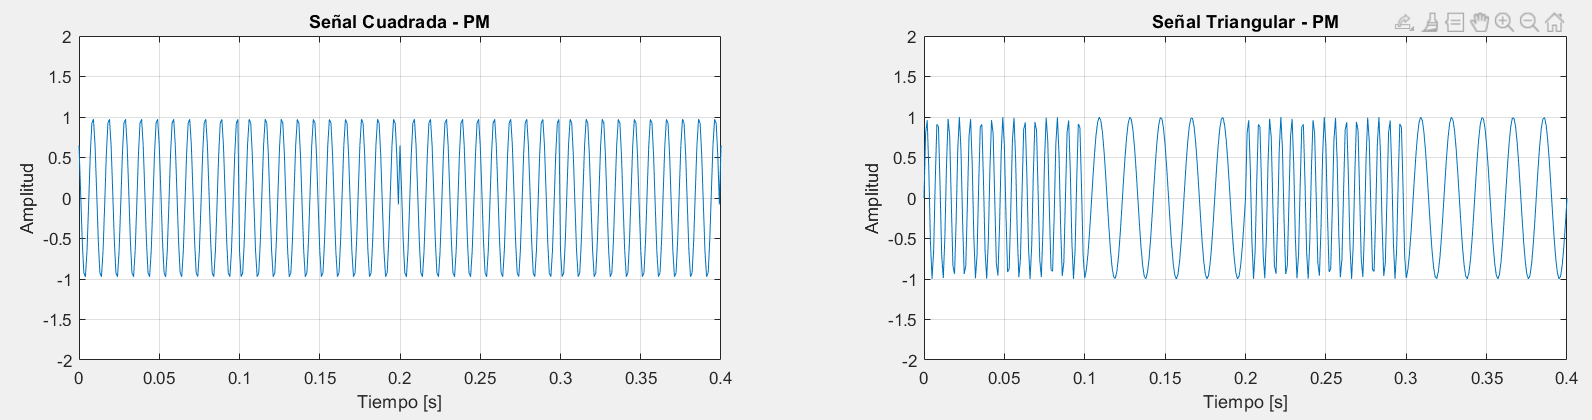
\includegraphics[width=0.5\textwidth]{media/modulacion-pm}
		\caption{Modulación PM}
		\label{fig:modulacion-pm}
	\end{figure}
	
	Finalmente este proceso emulado en el software MATLAB obtiene la siguiente respuesta mostrada en la figura \ref{fig:modulacion-pm} en la cual se puede apreciar un cambio significativo de fase para la integral de la señal de información o cuando este procedimiento se aplica en la señal triangular.
	
	\section{ Modulación FM}
	
	En la modulación en frecuencia, la variación de la señal moduladora (información) guarda una relación directa con la frecuencia instantánea, resultando este procedimiento en un variación de frecuencia que depende de la integral de la señal de información, permitiendo variaciones de frecuencia sin alterar significativamente la fase en la portadora, la definición matemática de una señal FM se define en \ref{eq:mod-fm} según la relación citada \cite{stremler2006}.
		
	\begin{equation}
		\phi_{FM}(t) = Asin( \omega_c t + \int_0^t k_f f(\tau)\, d\tau + \theta_0\ )
		\label{eq:mod-fm}
	\end{equation}
	
	Finalmente para resultados simulados de este procedimiento se muestran en la figura \ref{fig:modulacion-fm-sim}
	
	\begin{figure}[h]
		\centering
		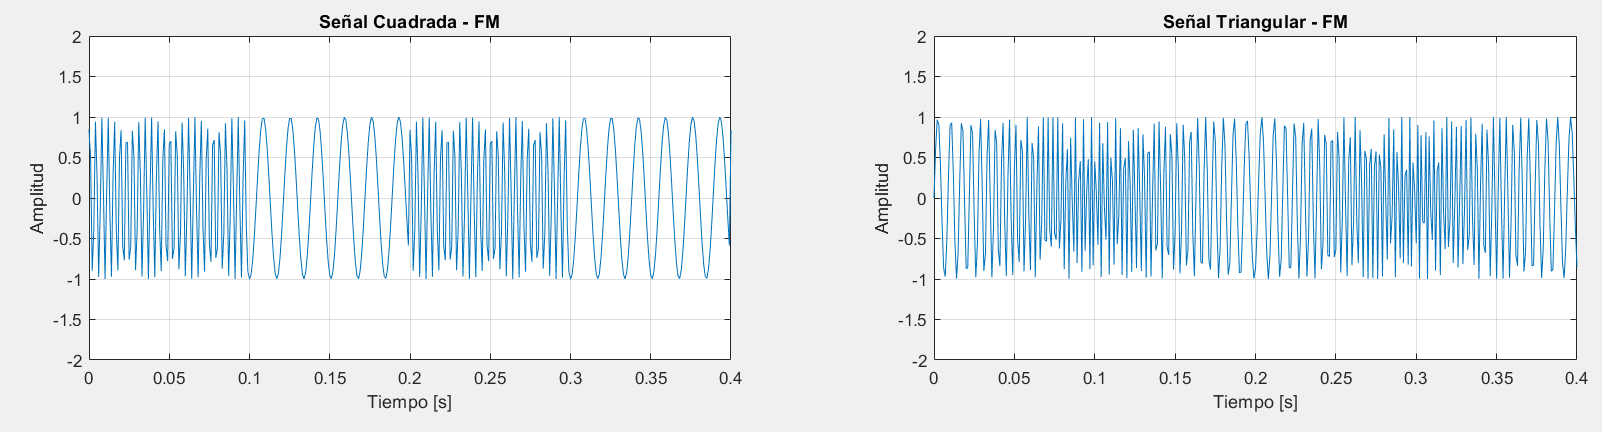
\includegraphics[width=0.5\textwidth]{media/modulacion-fm-sim}
		\caption{Modulación FM}
		\label{fig:modulacion-fm-sim}
	\end{figure}
	
	Y en la cual se puede destacar que la modulación FM de la señal cuadrada se asemeja a la modulación PM de la señal triangular, lo cual se detallará en la siguiente sección.
	
	\section{Relación entre ambos tipos de modulación}
	
	Una clara relación entre este tipo de modulaciones se puede apreciar en la figura \ref{fig:relacionpmfm} en la cual se puede apreciar que la señal triangular modulada en PM guarda cierta relación con la señal cuadrada modulada en FM debido a que una modulación FM integra la señal de información para su proceso.
	
	De este análisis se puede destacar que una señal FM aunque más común resulta un proceso más caro debido a que requiere una mayor cantidad de componentes para su implementación, sin embargo sus beneficios como su alta inmunidad al ruido la convirtieron en un método ideal para la transmisión de radio.
	
	Y el código asociado para realizar las comparaciones se puede apreciar en el bloque de código \ref{lst:mod-pm-fm}
	
	\section{Código en MATLAB}
	
	\begin{lstlisting}[numbers=none, caption="Generación de una señal PM y FM", label=lst:mod-pm-fm]
		clc, clear, close all;
		
		%% GENERACION DE LAS SENALES
		clc; clear; close all;
		
		f = 5;               % Frecuencia de la senal (Hz)
		T = 1/f;             % Periodo
		Fs = 1000;           % Frecuencia de muestreo
		Ts = 1/Fs;
		t = 0: Ts : 2*T;      % Vector de tiempo para dos periodos
		
		
		% SENAL CUADRADA
		ft1 = square(2*pi*f*t);
		
		% SENAL TRIANGULAR
		ft2 = 1 + sawtooth(2*pi*f*t, 0.5);  % Ciclo de subida y bajada simetrico
		
		
		%% MODULACION PM Y FM
		
		% PORTADORA
		A = 1;
		fc = 100;
		kp = 15;
		
		% SENAL PM
		fi1 = A*sin( 2*pi*fc*t + kp*ft1);
		fi2 = A*sin( 2*pi*fc*t + kp*ft2);
		
		% SENAL FM
		fi3 = A*sin( 2*pi*fc*t + cumsum(ft1));
		fi4 = A*sin( 2*pi*fc*t + cumsum(ft2));
		
		%% GRAFICAS Y RESULTADOS
		figure;
		subplot(1, 2, 1);
		plot(t, ft1);
		title("Senal Cuadrada");
		
		subplot(1, 2, 2);
		plot(t, ft2);
		title("Senal Triangular");
		
		figure;
		subplot(2,2,1);
		plot(t, fi1);
		title('Senal Cuadrada - PM');
		xlabel('Tiempo [s]');
		ylabel('Amplitud');
		ylim([-2 2]);
		grid on;
		hold off;
		
		subplot(2,2,2);
		plot(t, fi2);
		title('Senal Triangular - PM');
		xlabel('Tiempo [s]');
		ylabel('Amplitud');
		ylim([-2 2]);
		grid on;
		hold off;
		
		subplot(2, 2, 3);
		plot(t, fi3);
		title('Senal Cuadrada - FM');
		xlabel('Tiempo [s]');
		ylabel('Amplitud');
		ylim([-2 2]);
		grid on;
		hold off;
		
		subplot(2, 2, 4);
		plot(t, fi4);
		title('Senal Triangular - FM');
		xlabel('Tiempo [s]');
		ylabel('Amplitud');
		ylim([-2 2]);
		grid on;
		hold off;
	\end{lstlisting}
	
	\bibliographystyle{IEEEtran}
	\bibliography{biblio}
\end{document}
